% Results section of holding_prm_report.tex (input from there).
% Every table body and every \Prm... number is written by
% docs/figures/make_prm_figures.py from the saved runs under <root>/prm/.

\subsection{What was run}

All runs used the benchmark's library \code{cdfm_v1} and its trimmed scenes
(the scene key and git state are in each run's provenance record), the
calibrated ssik solvers, eight worker
processes on the 16-thread workstation (no benchmark batch was running), and the
defaults of Section~\ref{sec:params} unless stated.
\begin{itemize}[nosep]
  \item \textbf{B18, goal 2} --- the goal whose 807 surveyed starts the BiRRT
        was run on in full (experiment 2, batch \code{20260929_1756}: two seeds
        per start, \PrmBirrtSolvedStarts{} of \PrmBirrtStarts{} starts solved at
        least once). Four roadmaps, with node budgets of 500, 1000, 2000 and
        4000 sampled nodes, all anchored on goal 2 with 40 anchor starts (81
        anchors in all: home, the 7 goal pairs, and 73 start configurations).
        Each roadmap was asked two separate questions, i.e.\ two queries on the
        same roadmap: one whose start set is only starts 0 and 12 (night 1:
        start 0 solved by 0 of 10 seeds, start 12 by 6 of 10), and one whose
        start set is all 807 starts.
  \item \textbf{B18, 2000 nodes, variations} --- seeds 1 and 2, every IK branch
        kept per draw, and no start--goal line draws.
  \item \textbf{B3, goals 4, 11 and 16} --- one 2000-node roadmap anchored on
        all three goals, queried per goal with the three night-1 starts.
\end{itemize}
Run folders are \path{<root>/prm/B18_g2_n<budget>/},
\path{B18_g2_n2000_<variation>/} and \path{B3_g4-11-16_n2000/}; the logs are in
\path{<root>/prm/logs/}.

\subsection{How fast a joint-space line leaves the holding surface}

\begin{figure}[h]
\centering
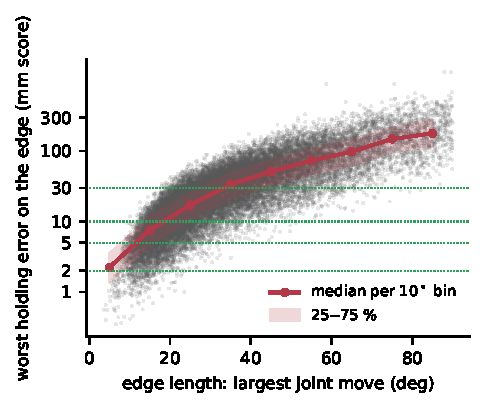
\includegraphics[width=0.52\linewidth]{figures/prm_viol_vs_length.pdf}
\caption{Worst holding error (score, Eq.~\ref{eq:score}) of every free edge of the
\PrmLargestBudget-node B18 roadmap against the edge's largest joint move. Dotted
lines: the four query tolerances.}
\label{fig:viol}
\end{figure}

Figure~\ref{fig:viol} is the single most important measurement of the pilot,
because it fixes how dense a roadmap has to be. Both ends of every edge hold the
bar exactly, yet the straight line between them does not: the median worst error
is \PrmMedianScoreShort\,mm for edges shorter than $20^\circ$ and
\PrmMedianScoreLong\,mm for edges of $60^\circ$ and more. For the short edges
that matter at small tolerances, sort the free edges by length (largest joint
move) into three narrow bins and take the median worst holding error in each:
\begin{center}
\footnotesize
\begin{tabular}{@{}lrrr@{}}
\toprule
edge length (largest joint move, deg) & 2.5--7.5 & 7.5--12.5 & 12.5--17.5 \\
free edges in the bin (count) & 51 & 642 & 2683 \\
median worst holding error (mm) & 1.0 & 3.6 & 6.9 \\
\bottomrule
\end{tabular}
\end{center}
In words: an edge of about $5^\circ$ drifts about 1\,mm from the holding surface
at its worst point; an edge as long as the continuity step $\tau = 10^\circ$
drifts about 3.6\,mm. Over this range the error grows roughly in proportion to the
length rather than with its square, so the roadmap's edges are far from the
regime where a straight chord hugs the curved holding surface. Two consequences
follow. First, a sub-2\,mm path needs a chain of edges of about $5^\circ$ each;
a roadmap sampled freely in twelve dimensions does not supply that density, so
the gaps below are best read as \emph{upper bounds} on how close a start is to
the goal set. Second, the holding error, not collision, is what limits a
joint-space roadmap: \PrmFreeEdgeShareLargest\,\% of candidate edges are
collision-free, but only 1.1\,\% of those free edges stay within 2\,mm, 7.5\,\%
within 5\,mm, 21\,\% within 10\,mm and 57\,\% within 30\,mm.

\subsection{The roadmaps and what they cost}

\begin{table}[h]
\centering
\footnotesize
\setlength{\tabcolsep}{3pt}
\caption{The four B18 roadmaps (goal-2 anchors, seed 0, 8 workers), one column
per node budget. A draw is one draw of the driving arm's six joints, followed by
one IK call for the other arm. A component is a set of nodes joined by
collision-free edges; the anchor rows say how many of the 7 goal anchors and the
73 start anchors sit in the largest one.}
\label{tab:build}
\begin{tabular}{@{}>{\raggedright\arraybackslash}p{6.8cm} rrrr@{}}
\toprule
node budget & 500 & 1000 & 2000 & 4000 \\
\midrule
sampled nodes kept: the node budget (count) & 500 & 1000 & 2000 & 4000 \\
all nodes, anchors included (count) & 581 & 1081 & 2081 & 4081 \\
driver-arm draws, one IK call each (count) & 2656 & 5344 & 10688 & 21408 \\
collision checks, sampling and edges together (count) & 11818 & 23969 & 47606 & 89047 \\
candidate edges measured (count) & 2922 & 6094 & 13028 & 26908 \\
collision-free edges (count) & 2657 & 5586 & 12000 & 25056 \\
components: separate islands of the free graph (count) & 71 & 90 & 125 & 173 \\
nodes in the largest component (count) & 262 & 525 & 1285 & 2557 \\
goal anchors in the largest component & 3 of 7 & 3 of 7 & 7 of 7 & 7 of 7 \\
start anchors in the largest component & 24 of 73 & 25 of 73 & 27 of 73 & 27 of 73 \\
\midrule
sampling time (s, wall clock) & 12 & 16 & 24 & 40 \\
edge measuring time (s, wall clock) & 28 & 74 & 103 & 181 \\
whole build (s, wall clock) & 51 & 100 & 138 & 232 \\
edge phase speed-up (worker-seconds per wall-second) & 7.4 & 7.8 & 7.9 & 8.0 \\
\bottomrule
\end{tabular}

\end{table}

\begin{figure}[h]
\centering
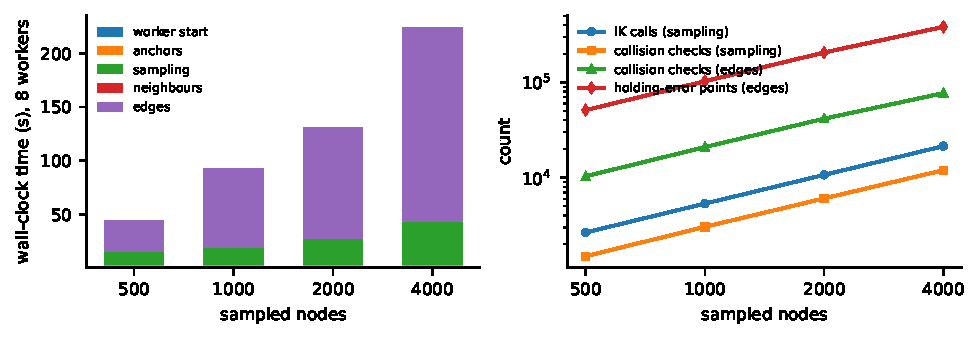
\includegraphics[width=\linewidth]{figures/prm_cost.pdf}
\caption{Left: where the build time goes. Right: the work counted, against the node budget.}
\label{fig:cost}
\end{figure}

\paragraph{Counting queries, as the meeting asked.}
Every build cost one analytical IK call per draw, and the sampler kept about one
node in four and a half draws: of the 21\,408 draws of the 4000-node build, 56\,\%
were reachable by the other arm, and 39\,\% of those were collision-free. The line
mode was by far the most productive (31\,\% of its draws kept, against 17\,\% for
the Gaussian and 5\,\% for the box), which is why it carries half the mix. The
edge phase then dominates: 77\,076 collision checks for 26\,908 edges, of which
1852 (6.9\,\%) collide. In worker time, collision checking was most of the
whole build (93\,\%: 1571 of 1680 worker-seconds at 4000 nodes, 15.7--17.9\,ms per check)
and IK 2.7\,\% (2.1\,ms per call); the 382\,241 holding-error points cost
nothing measurable. This inverts the pilot plan's expectation that IK would be
the expensive operation: here it is the full-cell compas\_fab check, exactly as
in the BiRRT's own profile. The GPU question is therefore a question about
batched collision checking, not about IK.

\paragraph{Parallel speed-up.}
Edge checking ran at 7.4--8.0 worker-seconds per wall-second on eight workers
(Table~\ref{tab:build}), i.e.\ essentially linearly; sampling reached 6.0 at 4000
nodes and less on small budgets, where a round is only a few chunks. The query's
endpoint expansion (38\,384 branch pairs collision-checked for the 807 starts)
ran at 7.2 and the endpoint edges at 7.7. The whole 4000-node build took
232\,s of wall time.

\paragraph{What an ``all-starts'' query is, and why it takes 200\,s.}
An all-starts query takes all 807 library start poses of the goal as its start
set and gives each of them an exact gap. It is a survey of the start poses, not
one planning query: on the same roadmap, the query with only starts 0 and 12
took 8.9\,s. The all-starts query took 208--229\,s whatever the roadmap size;
for the 4000-node roadmap the 212\,s split as follows.
\begin{center}
\footnotesize
\begin{tabular}{@{}>{\raggedright\arraybackslash}p{4.3cm} r >{\raggedright\arraybackslash}p{8.3cm}@{}}
\toprule
phase & time (s) & what it depends on \\
\midrule
solve and collision-check the start poses (38\,384 branch pairs) & 73 & only the start poses and the scene: can be done once and stored \\
holding error of the endpoint edges (99\,161 edges) & 28 & start poses and roadmap; not the goal \\
lazy gap verification (\PrmVerifyRounds{} rounds) & 104 & the goal; about half is the 0.64\,s spanning-tree search repeated every round, the rest is collision-checking \PrmLazyChecked{} edges (1231 blocked) \\
paths per tolerance & 3 & the goal \\
\bottomrule
\end{tabular}
\end{center}
So a night of precomputation can remove nearly all of it: with the start poses
and their edges solved and collision-checked once per roadmap, the verification
loop ends after its first round. Section~\ref{sec:precompute} builds and times
exactly this.

\paragraph{Lazy checking is exact in practice too.}
On the smoke roadmap (bar B3, 333 nodes, 380 starts) the same query was run with
endpoint edges checked lazily and eagerly: the gap of every one of the 380
starts (its smallest gap over all its branch pairs and turns) is the same both
ways, and the lazy query took 151\,s against 593\,s (two workers).

\subsection{Starts 0 and 12, and all 807 starts, against the node budget}

\begin{table}[h]
\centering
\footnotesize
\setlength{\tabcolsep}{3.5pt}
\caption{What each B18 roadmap answers, one column per node budget. The upper rows
come from the query whose start set is starts 0 and 12 only; the lower rows from
the query over all 807 starts. A gap is in mm of holding error (rotation folded
in at $0.4^\circ$ per mm); $\infty$: no route of free edges to any goal node.}
\label{tab:query}
\begin{tabular}{@{}>{\raggedright\arraybackslash}p{6.8cm} rrrr@{}}
\toprule
node budget & 500 & 1000 & 2000 & 4000 \\
\midrule
start 0: gap, best over its branch pairs and turns (mm) & 82.6 & 41.8 & 41.4 & 21.3 \\
start 0: gap of its library configuration alone (mm) & $\infty$ & $\infty$ & $\infty$ & $\infty$ \\
start 12: gap, best over its branch pairs and turns (mm) & 7.9 & 5.7 & 5.1 & 4.5 \\
start 12: gap of its library configuration alone (mm) & 22.1 & 29.2 & 29.2 & 24.2 \\
\midrule
all 807 starts: smallest gap (mm) & 7.9 & 5.7 & 4.2 & 2.9 \\
starts that reach the goal set at all (count of 807) & 650 & 657 & 657 & 657 \\
median gap of the starts that reach it (mm) & 49.4 & 41.8 & 30.5 & 24.3 \\
starts with a gap of at most 2 mm (count) & 0 & 0 & 0 & 0 \\
starts with a gap of at most 5 mm (count) & 0 & 0 & 1 & 11 \\
starts with a gap of at most 10 mm (count) & 13 & 17 & 24 & 36 \\
starts with a gap of at most 30 mm (count) & 114 & 115 & 171 & 462 \\
all-starts query time (s, wall clock) & 208 & 208 & 229 & 212 \\
\bottomrule
\end{tabular}

\end{table}

\begin{figure}[h]
\centering
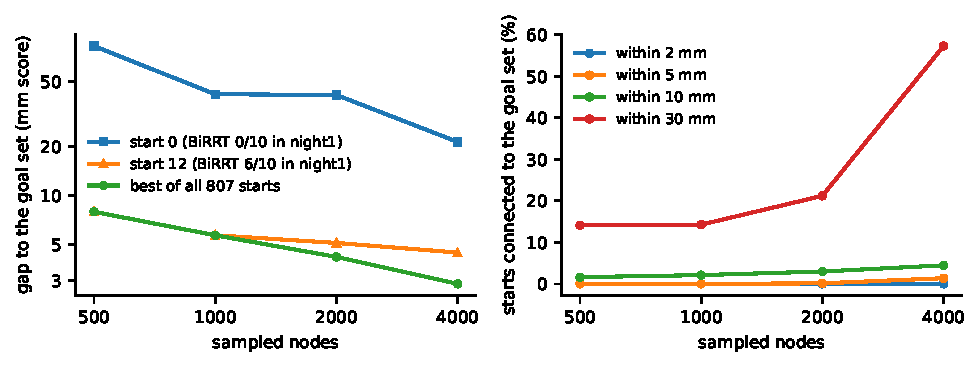
\includegraphics[width=\linewidth]{figures/prm_budget.pdf}
\caption{Left: gap to the goal set against the node budget for start 0, start 12 and
the best of all starts. Right: share of the 807 starts that reach the goal set within
each tolerance.}
\label{fig:budget}
\end{figure}

Three things stand out in Table~\ref{tab:query} and Fig.~\ref{fig:budget}.

\emph{Start 12 is near-feasible, start 0 is not.} Start 12, which the BiRRT
solved with 6 of 10 seeds in night 1, reaches the goal set within 7.9\,mm on the
smallest roadmap and within 4.5\,mm on the largest. Start 0, solved by none of
10 seeds, sits at 82.6\,mm on 500 nodes and still 21.3\,mm on 4000 nodes. The
reason is local: on the 2000-node roadmap, the 11--20 sampled nodes drawn around
start 0's two anchors ended up a median $96$--$121^\circ$ away from it (their
other arm lands on a distant IK branch, or they collide), and only two nodes lie
within $30^\circ$ of it; around start 12 the same numbers are $71$--$73^\circ$
and 13--28 nodes. Start 0's gap on that roadmap is set by three long edges
within the first five steps out of it ($45$--$52^\circ$, 31--41\,mm), not by
anything near the goal.

\emph{The library's own start configuration is often the wrong one.} For both
starts the gap of the library configuration alone (the rows ``gap of its library
configuration alone'' in Table~\ref{tab:query}) is much
larger than the best over all branch pairs and turns; for start 0 it is
unreachable at every budget. Over all starts, a different branch pair or turn
beat the library configuration for \PrmBetterBranchStarts{} of the
\PrmReachableStarts{} reachable starts, and the best node sat on the home turn
for most of them (Table~\ref{tab:turns}). This is the quantitative form of the
meeting's worry about start/goal branch pairing: fixing the start configuration
before searching throws away most of the useful connections.

\emph{More nodes help, slowly.} The best gap over all starts falls from 7.9 to
2.9\,mm from 500 to 4000 nodes, the median over starts from 49 to 24\,mm, and the
number of starts within 30\,mm from 114 to 462 (the least stable of these
numbers: Table~\ref{tab:ablation} shows it ranging from 171 to 405 across seeds
at 2000 nodes). No start reaches the goal set
within 2\,mm at any budget. Exactly the same 150 starts are unreachable at 1000,
2000 and 4000 nodes: their start nodes do have edges, but into clusters of the roadmap that no
edge of at most $90^\circ$ joins to the goal's component (the 4000-node roadmap
has 173 components); 136 of them are ``broken'' starts.

\begin{table}[h]
\centering
\footnotesize
\caption{The turn of each reachable start's best node (4000-node roadmap).}
\label{tab:turns}
\begin{tabular}{@{}lr@{}}
\toprule
turn of the best node & starts \\
\midrule
\tablerows{figures/prm_table_turns.tex}
\bottomrule
\end{tabular}
\end{table}

\subsection{Which starts are near the goal: classes, carry anchors, and the BiRRT}

\begin{table}[h]
\centering
\footnotesize
\caption{All 807 starts of B18 goal 2 on the \PrmLargestBudget-node roadmap, by the
library's straight-line class and by the BiRRT's outcome in experiment 2. ``reach'':
starts with any route to the goal set; the last four columns count starts within each
tolerance (mm).}
\label{tab:classes}
\begin{tabular}{@{}lrrrrrrr@{}}
\toprule
group & starts & reach & median gap & $\le$2 & $\le$5 & $\le$10 & $\le$30 \\
\midrule
\tablerows{figures/prm_table_classes.tex}
\bottomrule
\end{tabular}
\end{table}

\begin{table}[h]
\centering
\footnotesize
\caption{The same starts by carry anchor. The last column counts the starts of each
anchor that the BiRRT solved at least once in experiment 2.}
\label{tab:carry}
\begin{tabular}{@{}lrrrrrr@{}}
\toprule
carry anchor & starts & reach & median gap & $\le$10 & $\le$30 & BiRRT solved \\
\midrule
\tablerows{figures/prm_table_carry.tex}
\bottomrule
\end{tabular}
\end{table}

\begin{figure}[h]
\centering
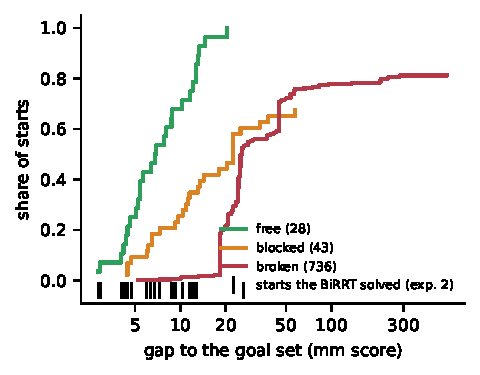
\includegraphics[width=0.52\linewidth]{figures/prm_gap_by_class.pdf}
\caption{Share of starts whose gap is below a value, per library class (starts with no
route are the missing share at the right). Ticks under the axis: the gaps of the
starts the BiRRT solved in experiment 2.}
\label{fig:classes}
\end{figure}

\paragraph{The roadmap ranks the starts the way the BiRRT did.}
The roadmap never ran the BiRRT and knows nothing about its results, yet the
starts the BiRRT solved at least once in experiment 2 are the ones the roadmap
puts closest to the goal set: all \PrmBirrtSolvedStarts{} of them are reachable,
their median gap is \PrmSolvedMedianGap\,mm against 24.3\,mm for the starts it
never solved, 15 of them are within 10\,mm and all 21 within 30\,mm
(Table~\ref{tab:classes}). The five starts with the smallest gaps were all solved
by the BiRRT, and seven of the best ten. The library's straight-line classes are
ordered the same way (medians 6.8, 11.5 and 24.4\,mm for free, blocked and
broken). The ranking is not perfect in the other direction: 21 of the 36 starts
within 10\,mm were never solved in experiment 2, but that batch ran only two seeds
per start, and one of those 21 is start 12, which night 1 solved with 6 of 10
seeds.

\paragraph{The carry anchor matters most.}
Table~\ref{tab:carry} is the clearest single result. Every start the BiRRT solved
is a ``back'' carry pose, and so is every start within 10\,mm of the goal set; no
horizontal or vertical start comes within 10\,mm, and the vertical ones have a
median gap of 57\,mm. The benchmark's night-1 analysis found that production's
start derivation always picks the horizontal anchor and succeeds 2.7\,\% of the
time from it. For this goal the roadmap says why: from a horizontal carry pose no
route of short joint-space steps reaches any of the goal's branch pairs.

\subsection{The best path}

\begin{figure}[h]
\centering
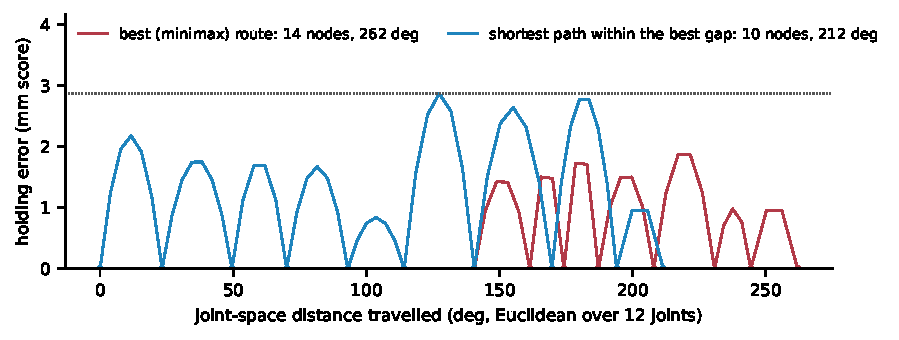
\includegraphics[width=\linewidth]{figures/prm_profile.pdf}
\caption{Holding error along the best route of the \PrmLargestBudget-node roadmap
(start \PrmBestStart) and along the shortest path within the same gap. Dots: roadmap
nodes, where the error is zero. Dotted line: the gap.}
\label{fig:profile}
\end{figure}

The best route of the \PrmLargestBudget-node roadmap starts at start
\PrmBestStart{} (a back, free-class start the BiRRT solved), on branch pair
\PrmBestStartPair{} and the \PrmBestStartTurn{} turn --- not its library
configuration --- and ends at the goal's branch pair \PrmBestGoalLibraryPair{}
(library numbering). It has \PrmBestRouteNodes{} nodes and travels
\PrmBestRouteLength\,rad in joint space, with no joint moving more than
\PrmBestRouteMaxStep$^\circ$ between the dense points of the profile, so it
contains no branch flip by construction. Its worst holding error is
\PrmBestGap\,mm. Figure~\ref{fig:profile} shows what that number is made of: the
error rises from zero at each node to a peak in the middle of each edge and
falls back to zero at the next node, and the peaks are all of similar height.
Only two of the thirteen edges peak above 2\,mm (at 2.2 and 2.9\,mm); the others
peak between 0.8 and 1.9\,mm. There is no plateau and no single dominant spike:
this is a resolution limit of the roadmap, not a sign that the start and the
goal sit on disconnected sheets. Replacing those two edges by shorter ones ---
locally resampling around them, as the plan's refinement step proposes --- is
all that stands between this route and a sub-2\,mm path. The filtered searches
tell the same story from the other side: within 5\,mm eleven starts connect, the
shortest such path (7 nodes, from start 312, another BiRRT-solved start) has a
worst error of 4.6\,mm, and within 10 and 30\,mm the shortest paths have 5--6
nodes.

\begin{figure}[h]
\centering
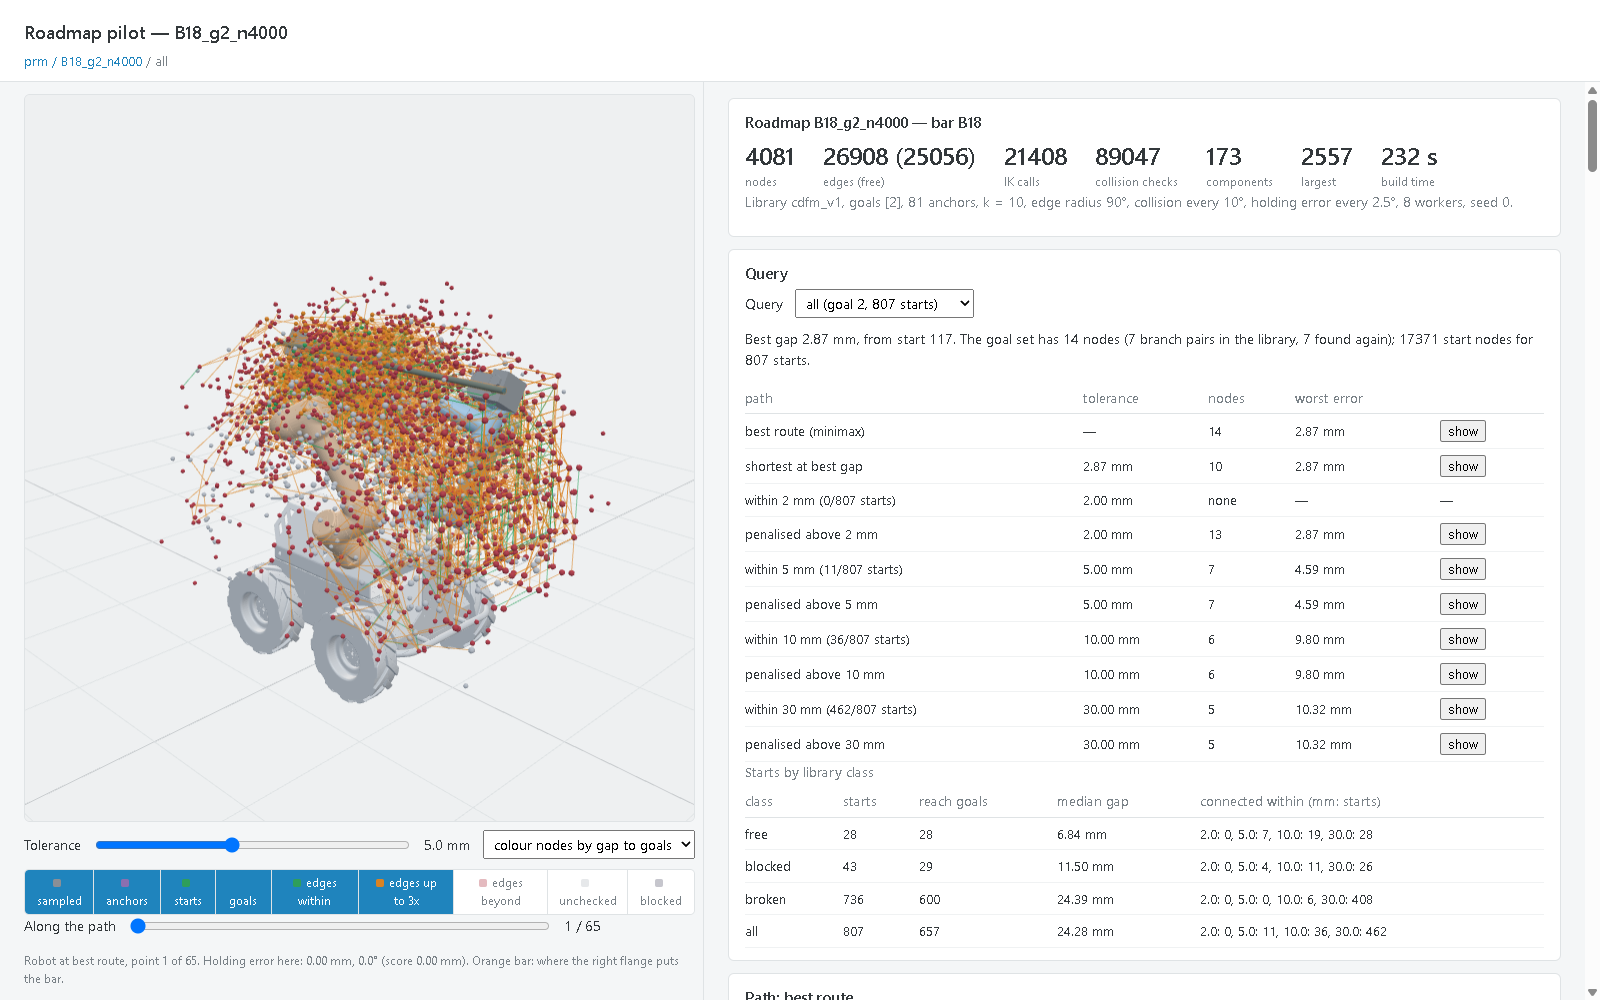
\includegraphics[width=\linewidth]{figures/prm_dashboard.png}
\caption{The roadmap page on the 4000-node B18 roadmap and the all-starts query:
nodes at the midpoint of the two flanges, coloured by their gap to the goal set at
the 5\,mm slider setting, edges coloured by their worst holding error, the robot
posed at the first point of the best route.}
\label{fig:dashboard}
\end{figure}

\subsection{Seeds and two sampler choices}

\begin{table}[h]
\centering
\footnotesize
\setlength{\tabcolsep}{3.5pt}
\caption{The 2000-node B18 roadmap under three seeds and two sampler changes, one
column per roadmap; rows as in Tables~\ref{tab:build} and~\ref{tab:query}.}
\label{tab:ablation}
\begin{tabular}{@{}>{\raggedright\arraybackslash}p{6.2cm} rrrrr@{}}
\toprule
roadmap & \shortstack{seed 0\\(default)} & seed 1 & seed 2 & \shortstack{every IK\\branch kept} & \shortstack{no line\\draws} \\
\midrule
sampled nodes kept: the node budget (count) & 2000 & 2000 & 2000 & 2000 & 2000 \\
all nodes, anchors included (count) & 2081 & 2081 & 2081 & 2081 & 2081 \\
driver-arm draws, one IK call each (count) & 10688 & 9280 & 10304 & 2272 & 16768 \\
collision checks, sampling and edges together (count) & 47606 & 46198 & 46252 & 45350 & 58085 \\
candidate edges measured (count) & 13028 & 12983 & 12896 & 9500 & 11929 \\
collision-free edges (count) & 12000 & 11871 & 11909 & 8611 & 10174 \\
components: separate islands of the free graph (count) & 125 & 139 & 148 & 296 & 200 \\
nodes in the largest component (count) & 1285 & 1044 & 1034 & 755 & 1460 \\
goal anchors in the largest component & 7 of 7 & 3 of 7 & 3 of 7 & 3 of 7 & 3 of 7 \\
start anchors in the largest component & 27 of 73 & 24 of 73 & 24 of 73 & 23 of 73 & 48 of 73 \\
\midrule
sampling time (s, wall clock) & 24 & 19 & 24 & 21 & 25 \\
edge measuring time (s, wall clock) & 103 & 82 & 98 & 78 & 97 \\
whole build (s, wall clock) & 138 & 114 & 133 & 110 & 132 \\
edge phase speed-up (worker-seconds per wall-second) & 7.9 & 7.9 & 7.9 & 7.8 & 7.9 \\
\midrule
start 0: gap, best over its branch pairs and turns (mm) & 41.4 & 33.0 & 23.5 & 73.2 & 38.2 \\
start 0: gap of its library configuration alone (mm) & $\infty$ & $\infty$ & $\infty$ & $\infty$ & $\infty$ \\
start 12: gap, best over its branch pairs and turns (mm) & 5.1 & 3.9 & 5.0 & 5.3 & 13.7 \\
start 12: gap of its library configuration alone (mm) & 29.2 & 11.2 & 34.1 & 31.1 & 29.1 \\
\midrule
all 807 starts: smallest gap (mm) & 4.2 & 3.8 & 5.0 & 5.2 & 13.7 \\
starts that reach the goal set at all (count of 807) & 657 & 651 & 658 & 658 & 650 \\
median gap of the starts that reach it (mm) & 30.5 & 24.3 & 24.5 & 44.0 & 25.5 \\
starts with a gap of at most 2 mm (count) & 0 & 0 & 0 & 0 & 0 \\
starts with a gap of at most 5 mm (count) & 1 & 4 & 3 & 0 & 0 \\
starts with a gap of at most 10 mm (count) & 24 & 25 & 27 & 16 & 0 \\
starts with a gap of at most 30 mm (count) & 171 & 400 & 405 & 112 & 406 \\
all-starts query time (s, wall clock) & 229 & 236 & 205 & 203 & 188 \\
\bottomrule
\end{tabular}

\end{table}

\paragraph{Seeds.} Across three seeds at 2000 nodes the best gap is 3.8--5.0\,mm,
start 12's gap 3.9--5.1\,mm, and 24--27 starts are within 10\,mm: these numbers
are stable. Start 0's gap (23.5--41.4\,mm) and the count within 30\,mm (171,
400, 405) are not; seed 0 happens to be the unlucky one for both, so the 30\,mm
counts of Table~\ref{tab:query} should be read with a spread of that size.

\paragraph{Keeping every IK branch} makes each draw yield more nodes, and that
is exactly why it does worse at a fixed node budget. The budget counts nodes,
not draws: 2000 nodes came from only 2272 draws (about 10\,000 with
$\beta = 1$), so four times fewer distinct bar poses were tried, and each was
copied onto postures far from each other (flipped elbows and wrists, a median
$182^\circ$ from the anchor on the smoke roadmap). Such copies find few
neighbours within $90^\circ$, so the roadmap has \emph{fewer} edges, not more
(3500 fewer), falls into 296 components, and every quality number is worse
(median gap 44\,mm, 16 starts within 10\,mm, 112 within 30\,mm). The effort is
spread over many branch sheets instead of filling the one or two that connect
the starts to the goal. Section~\ref{sec:e4} gives it the same number of draws.

\paragraph{Without the start--goal line draws} the roadmap still covers the
space (406 starts within 30\,mm, similar to the default seeds) but loses all
precision: no start comes within 10\,mm, and the best gap rises to 13.7\,mm.
This is not about the start itself. A start's gap is the worst edge anywhere
on its best route to the goal, not something measured at the start; line
draws put closely spaced nodes all along the corridor between starts and goal
pairs, and without them the middle of every route is made of long edges, and a
long edge drifts far from the holding surface (Fig.~\ref{fig:viol}). The
near-feasible routes of Fig.~\ref{fig:profile} are made almost entirely of
line-draw nodes; they are what the roadmap's precision rests on. Line draws are
also the most productive per draw (31\,\% kept, against 17\,\% for the Gaussian
and 5\,\% for the box, at 4000 nodes), which is why the no-line roadmap needed
16\,768 draws for the same 2000 nodes.

\subsection{From roadmap routes to exact paths (E2)}
\label{sec:e2}

\begin{table}[h]
\centering
\footnotesize
\setlength{\tabcolsep}{3pt}
\caption{Refinement of the all-starts queries (Section~\ref{sec:refine}), one column per
roadmap or tracker setting. ``Exact path from a route within $t$'' means: some route all
of whose roadmap edges score at most $t$ was turned into waypoints that hold the bar
exactly, are collision-free and never move a joint more than $10^\circ$.}
\label{tab:refine}
\begin{tabular}{@{}>{\raggedright\arraybackslash}p{7.6cm} rrrrr@{}}
\toprule
refinement & \shortstack{4000 nodes\\knots $2.5^\circ$} & \shortstack{4000 nodes\\end nodes only} & \shortstack{2000 nodes\\seed 0} & \shortstack{2000 nodes\\seed 1} & \shortstack{2000 nodes\\seed 2} \\
\midrule
starts within 30 mm on the roadmap: the ones refined (count) & 462 & 462 & 171 & 400 & 405 \\
edges tracked (count) & 3329 & 3388 & 1091 & 2373 & 2735 \\
\quad of which the tracker turned into exact waypoints & 2737 & 2762 & 885 & 1961 & 2304 \\
\quad failed: no IK solution at some waypoint & 65 & 45 & 14 & 35 & 37 \\
\quad failed: a joint jumped more than $10^\circ$ & 136 & 119 & 25 & 98 & 104 \\
\quad failed: a corrected waypoint collides & 19 & 47 & 1 & 16 & 21 \\
\quad failed: changes elbow branch, so it cannot meet the next edge & 372 & 415 & 166 & 263 & 269 \\
edges re-tracked from a route's last waypoint at a node (count) & 0 & 0 & 0 & 0 & 0 \\
edges dropped because a route could not continue (count) & 1 & 2 & 0 & 0 & 0 \\
\midrule
starts with an exact path from a route within 2 mm, of those the roadmap brings within 2 mm & 0 of 0 & 0 of 0 & 0 of 0 & 0 of 0 & 0 of 0 \\
starts with an exact path from a route within 5 mm, of those the roadmap brings within 5 mm & 11 of 11 & 11 of 11 & 1 of 1 & 4 of 4 & 3 of 3 \\
starts with an exact path from a route within 10 mm, of those the roadmap brings within 10 mm & 34 of 36 & 33 of 36 & 24 of 24 & 25 of 25 & 27 of 27 \\
starts with an exact path from a route within 30 mm, of those the roadmap brings within 30 mm & 245 of 462 & 169 of 462 & 81 of 171 & 81 of 400 & 129 of 405 \\
\midrule
best start: smallest exact gap (mm) & 2.87 & 2.87 & 4.20 & 3.78 & 4.97 \\
\quad its start index & 117 & 117 & 227 & 313 & 12 \\
\quad waypoints of its exact path (count) & 178 & 139 & 207 & 125 & 164 \\
\quad largest joint step between waypoints (deg) & 2.76 & 3.55 & 2.69 & 2.57 & 2.31 \\
\quad holding error of its waypoints (mm) & 4e-09 & 4e-09 & 4e-09 & 4e-09 & 4e-09 \\
refinement time (s, wall clock) & 1210 & 1085 & 483 & 858 & 902 \\
stored exact paths (one per start, plus the best and the shortest ones) passing the production repair at 2 mm steps & 249 of 249 & -- & -- & -- & -- \\
\bottomrule
\end{tabular}

\end{table}

\begin{figure}[h]
\centering
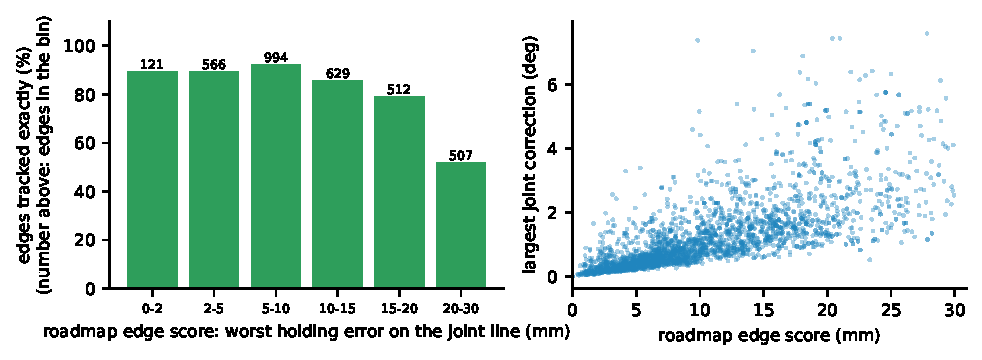
\includegraphics[width=\linewidth]{figures/prm_trackability.pdf}
\caption{Every edge the refinement of the 4000-node roadmap tracked. Left: share of
edges turned into exact waypoints, by the edge's roadmap score. Right: how far the
correction moved the joints away from the straight joint line.}
\label{fig:track}
\end{figure}

\paragraph{Within 10\,mm, almost every route becomes an exact path.} Of the
\PrmRoadmapTen{} starts the 4000-node roadmap brings within 10\,mm of the goal set,
\PrmExactTen{} have an exact path from a route within 10\,mm; within 5\,mm, all
\PrmRoadmapFive{} do; within 30\,mm, \PrmExactThirty{} of \PrmRoadmapThirty. The whole
refinement of the 807-start query took \PrmRefineSeconds\,s on eight workers
(\PrmRefineRounds{} tracking rounds, \PrmRefineEdges{} edges tracked). The best start
is the same as the roadmap's (start \PrmExactBestStart): its exact path has
\PrmExactBestWaypoints{} waypoints, holds the bar to $10^{-7}$\,m, and moves no joint
more than \PrmExactBestStep$^\circ$ between waypoints.

\paragraph{Why 10\,mm is a good working tolerance.} Fig.~\ref{fig:track} shows that an
edge's chance of tracking stays near 90\,\% up to 10\,mm (89\,\% under 5\,mm, 92\,\%
between 5 and 10\,mm; the failures there are mostly edges whose joint line passes a
stretched elbow, which no tolerance helps) and then falls: 86\,\% between 10 and
15\,mm, 79\,\% between 15 and 20\,mm, 52\,\% between 20 and 30\,mm. The joint correction
grows at about $0.1^\circ$ per mm of roadmap error (median over the tracked edges). So
up to 10\,mm the roadmap's routes are nearly as good as exact ones, and a 10\,mm roadmap
is the right thing to search before refining, as proposed. Of the \PrmRefineEdges{} tracked edges, \PrmRefineBranchChange{} changed
elbow branch, \PrmRefineContinuity{} hit the continuity gate, \PrmRefineIk{} met a pose
one arm cannot reach, and \PrmRefineCollision{} collided once corrected.

\paragraph{The same on other roadmaps, and why the knots matter.} On the three
2000-node roadmaps (seeds 0, 1, 2), every start within 10\,mm got an exact path (24 of
24, 25 of 25, 27 of 27); within 30\,mm, 81 of 171, 81 of 400 and 129 of 405
(Table~\ref{tab:refine}). So ``within 10\,mm on the roadmap'' reliably means ``an exact
path exists'', while within 30\,mm it is roughly a coin toss that depends on the
roadmap. Tracking a straight bar move between the two end nodes instead of following
the bar along the joint line (``end nodes only'') gives nearly the same answer within
10\,mm (33 of 36) but clearly fewer exact paths within 30\,mm (169 against 245): on
longer edges the bar's straight move strays further from the joint line, and more of
those edges change branch (415 against 372) or collide (47 against 19).

\paragraph{Exact paths from starts the BiRRT never solves.} \PrmExactHorizontal{}
horizontal starts have an exact path (from routes between 10 and 30\,mm), although the
BiRRT solved none of the 458 horizontal starts in experiment 2; \PrmExactBack{} back
starts do too, \PrmExactThirty{} in all, against the BiRRT's 21 (two seeds per
start). \PrmExactBirrtOverlap{} of the 21 starts the BiRRT
solved are among them. This qualifies the carry-anchor finding above: from a
horizontal carry pose no route stays within 10\,mm, but many routes within 30\,mm can
still be made exact.

\begin{table}[h]
\centering
\footnotesize
\caption{The production check of every stored exact path of the 4000-node refinement:
the production repair (\code{core.repair_joint_path}) re-solves each path at 2\,mm and
0.002\,rad bar steps with the production solver, gate and collision check.}
\label{tab:validation}
\begin{tabular}{@{}>{\raggedright\arraybackslash}p{8.0cm} rrrr@{}}
\toprule
carry anchor & back & horizontal & vertical & all \\
\midrule
starts within 30 mm on the roadmap (count) & 171 & 291 & 0 & 462 \\
starts with an exact path from the roadmap (count) & 81 & 164 & 0 & 245 \\
\quad passing the production repair at 2 mm steps & 81 & 164 & 0 & 245 \\
\quad failing it on a collision between the 1 cm waypoints & 0 & 0 & 0 & 0 \\
\quad failing it otherwise & 0 & 0 & 0 & 0 \\
\midrule
starts the BiRRT solved at least once in experiment 2 (count) & 21 & 0 & 0 & 21 \\
\quad of which the roadmap also gives a production-checked path & 20 & 0 & 0 & 20 \\
\bottomrule
\end{tabular}

\end{table}

\paragraph{The production check.} \PrmCheckPassed{} of the \PrmCheckPaths{} exact paths
pass the production repair unchanged (Table~\ref{tab:validation}; \PrmCheckSeconds\,s on
eight workers), \PrmCheckPassedHorizontal{} of them from horizontal starts and
\PrmCheckPassedBirrt{} from starts the BiRRT also solved: every path the refinement
returns is one the production planner would accept as is. Earlier versions of the
tracker passed 7 of 38, then 217 of 244, then 243 of 268 paths; the difference was
hidden branch hops near straight elbows, which the production walk at 2\,mm does not take
(Section~\ref{sec:refine}). Removing them also removes the starts whose only exact
route relied on such a hop, which is why the counts in Table~\ref{tab:refine} are
lower than in the first version (298 starts within 30\,mm then, \PrmExactThirty{} now;
within 10\,mm the count stayed at 34).

\subsection{Tightening routes: tube draws (way 2) and a seeded BiRRT (way 1) (E3)}
\label{sec:e3}

\begin{table}[h]
\centering
\footnotesize
\caption{The 4000-node refinement without and with three rounds of tube draws
(each round: 200 draws around the routes of the 20 starts with the largest exact gap
above 10\,mm).}
\label{tab:tube}
\begin{tabular}{@{}>{\raggedright\arraybackslash}p{7.4cm} rr@{}}
\toprule
refinement & without tube draws & with 3 tube rounds \\
\midrule
starts with an exact path from a route within 2 mm (count) & 0 & 20 \\
starts with an exact path from a route within 5 mm (count) & 11 & 86 \\
starts with an exact path from a route within 10 mm (count) & 34 & 120 \\
starts with an exact path from a route within 30 mm (count) & 245 & 245 \\
nodes added by tube draws (count) & 0 & 10099 \\
tube rounds run (count) & 0 & 3 \\
target starts improved, summed over rounds (count) & -- & 60 \\
refinement time (s, wall clock) & 1210 & 1888 \\
stored exact paths passing the production repair at 2 mm steps & 249 of 249 & 125 of 125 \\
\bottomrule
\end{tabular}

\end{table}

\begin{table}[h]
\centering
\footnotesize
\caption{The seeded BiRRT on the 24 starts still without any exact path after the tube
rounds (smallest roadmap gaps first; all have roadmap gaps under 30\,mm).}
\label{tab:birrt}
\IfFileExists{figures/prm_table_birrt.tex}{\begin{tabular}{@{}>{\raggedright\arraybackslash}p{7.4cm} rr@{}}
\toprule
seeded BiRRT & seeded with the exact chains & from the two ends only \\
\midrule
unresolved starts tried (count) & 24 & 24 \\
a path found (count) & 0 & 1 \\
\quad passing the production repair (count) & 0 & 1 \\
median time of a passing run (s) & -- & 15 \\
median IK solves of a passing run (count) & -- & 806 \\
of the starts tried, solved by the plain BiRRT in experiment 2 (count) & 0 & 0 \\
time limit per start (s) & 120 & 120 \\
\bottomrule
\end{tabular}
}{(missing)}
\end{table}

\paragraph{Tube draws work: the needed tolerance drops several-fold.} Drawing nodes in a
narrow tube ($5^\circ$) around a start's current route and searching again is the
refinement proposed in the meeting, and it does what was hoped
(Table~\ref{tab:tube}): with three rounds of about 3400 nodes each, the starts with an
exact path from a route within 10\,mm went from 34 to 120 (42 of them horizontal, none
before), within 5\,mm from 11 to 86, and within 2\,mm from none to 20. Every target start
improved in every round. The best route now needs only 0.89\,mm of roadmap tolerance
(start 206, whose roadmap gap was 23.4\,mm before the tubes). The tubes do not add
starts beyond the 245 that already had an exact path within 30\,mm: they tighten
routes, they do not create them. They cost 12 minutes on top of the 20-minute
refinement, and all 125 exact paths stored from the tube-refined routes pass the
production repair as well.

\paragraph{The seeded BiRRT does not bridge what the tracker cannot.} On the 24 starts
left without any exact path (Table~\ref{tab:birrt}), the BiRRT seeded with the
route's exact pieces found no path in 120\,s each; started from the two ends only,
with the same tube of samples, it found one (start 573, in 15\,s, and it passes the
production check). Of the 49 failed edges on these 24 routes, 30 are branch changes at a
stretched elbow (Section~\ref{sec:refine}) and 17 pass through poses one arm cannot
reach; a task-space tree grown from the exact pieces meets the same obstacles, so
seeding it with them does not help (it may even hurt: the trees start deep inside the
two branch sheets that do not meet). These are
the hardest starts of the goal, so the sample says little about the BiRRT in general,
but for this refinement the roadmap side (tubes) is clearly the better lever.

\subsection{Wider edges (E1) and every IK branch at the same number of draws (E4)}
\label{sec:e1}

\begin{table}[h]
\centering
\footnotesize
\setlength{\tabcolsep}{3pt}
\caption{E1: the 4000-node roadmap rebuilt with edges of up to $160^\circ$ (same
seed, so the same sampled nodes; only the edges differ). E4: every IK branch kept,
given about the same number of draws (10\,848) as the default 2000-node roadmap
(10\,688 draws, one branch per draw), next to the earlier every-branch roadmap that
stopped at 2000 nodes (2272 draws).}
\label{tab:e1e4}
\begin{tabular}{@{}>{\raggedright\arraybackslash}p{6.2cm} rrrrr@{}}
\toprule
roadmap & \shortstack{4000 nodes\\$90^\circ$ (ref.)} & \shortstack{4000 nodes\\$160^\circ$ (E1)} & \shortstack{every branch\\2272 draws} & \shortstack{every branch\\10k draws (E4)} & \shortstack{one branch\\10k draws (ref.)} \\
\midrule
sampled nodes kept: the node budget (count) & 4000 & 4000 & 2000 & 9400 & 2000 \\
all nodes, anchors included (count) & 4081 & 4081 & 2081 & 9481 & 2081 \\
driver-arm draws, one IK call each (count) & 21408 & 21408 & 2272 & 10848 & 10688 \\
collision checks, sampling and edges together (count) & 89047 & 101487 & 45350 & 232212 & 47606 \\
candidate edges measured (count) & 26908 & 29089 & 9500 & 56748 & 13028 \\
collision-free edges (count) & 25056 & 25928 & 8611 & 51717 & 12000 \\
components: separate islands of the free graph (count) & 173 & 68 & 296 & 533 & 125 \\
nodes in the largest component (count) & 2557 & 3873 & 755 & 5839 & 1285 \\
goal anchors in the largest component & 7 of 7 & 7 of 7 & 3 of 7 & 3 of 7 & 7 of 7 \\
start anchors in the largest component & 27 of 73 & 67 of 73 & 23 of 73 & 49 of 73 & 27 of 73 \\
\midrule
sampling time (s, wall clock) & 40 & 35 & 21 & 99 & 24 \\
edge measuring time (s, wall clock) & 181 & 226 & 78 & 658 & 103 \\
whole build (s, wall clock) & 232 & 272 & 110 & 769 & 138 \\
edge phase speed-up (worker-seconds per wall-second) & 8.0 & 6.0 & 7.8 & 6.0 & 7.9 \\
\midrule
start 0: gap, best over its branch pairs and turns (mm) & 21.3 & 21.3 & 73.2 & 21.8 & 41.4 \\
start 0: gap of its library configuration alone (mm) & $\infty$ & 648.9 & $\infty$ & $\infty$ & $\infty$ \\
start 12: gap, best over its branch pairs and turns (mm) & 4.5 & 4.5 & 5.3 & 4.3 & 5.1 \\
start 12: gap of its library configuration alone (mm) & 24.2 & 24.2 & 31.1 & 24.2 & 29.2 \\
\midrule
all 807 starts: smallest gap (mm) & 2.9 & 2.9 & 5.2 & 3.4 & 4.2 \\
starts that reach the goal set at all (count of 807) & 657 & 801 & 658 & 713 & 657 \\
median gap of the starts that reach it (mm) & 24.3 & 25.0 & 44.0 & 23.1 & 30.5 \\
starts with a gap of at most 2 mm (count) & 0 & 0 & 0 & 0 & 0 \\
starts with a gap of at most 5 mm (count) & 11 & 11 & 0 & 12 & 1 \\
starts with a gap of at most 10 mm (count) & 36 & 36 & 16 & 47 & 24 \\
starts with a gap of at most 30 mm (count) & 462 & 462 & 112 & 471 & 171 \\
all-starts query time (s, wall clock) & 212 & 553 & 203 & 340 & 229 \\
\bottomrule
\end{tabular}

\end{table}

\paragraph{E1: $160^\circ$ edges connect more starts, but only through useless
edges.} Widening the edge limit from $90^\circ$ to $160^\circ$ merged the roadmap
from 173 components into 68 and made 801 of the 807 starts reachable instead of
657. But the 144 newly reachable starts reach the goal set only through edges that
break the holding constraint by 220 to 1787\,mm (median 984\,mm; none within
100\,mm): a straight joint line of more than $90^\circ$ simply does not hold the bar.
Of the 657 starts reachable both ways, 11 got a smaller gap, all of them above
30\,mm before and after. Nothing within 30\,mm changed (best gap 2.87\,mm; 11, 36
and 462 starts within 5, 10 and 30\,mm), while the all-starts query took 553\,s
instead of 212\,s (272 verification rounds instead of 80). The $90^\circ$ limit
was not hiding useful connections; the islands it leaves apart are joined only by
moves no path can use.
\label{sec:e4}

\paragraph{E4: every IK branch is worth it per draw, not per second.} With the node
budget counting nodes, keeping every branch looked worse (Table~\ref{tab:ablation}).
Given the same number of draws as the one-branch roadmap, it is clearly better: 47
starts within 10\,mm and 471 within 30\,mm, against 24--27 and 171--405 for the three
one-branch seeds, and a best gap of 3.4\,mm against 3.8--5.0\,mm. That is about what
the one-branch roadmap reaches with twice the draws (4000 nodes: 36 and 462). But it
has 9481 nodes, 56\,748 candidate edges and 232\,000 collision checks, and took
769\,s to build against 232\,s for the 4000-node one-branch roadmap; its graph is
also more broken (533 components, only 3 of the 7 goal anchors in the largest).
Per collision check the one-branch roadmap is still ahead: 36 starts within 10\,mm
for 89\,000 checks, against 47 for 232\,000. The other branches help because they
are other routes to the same goal pairs, which is also the motivation for the
start and goal \emph{sets}.

\subsection{Re-calibrating the three carry poses (E5)}
\label{sec:e5}

The library's start poses come from three carry anchors that were never
calibrated; the horizontal one, for example, puts the grasp midpoint at
$x = 0.40$\,m, 19\,cm closer to the robot than the demo pose it was taken from.
The search (\path{holding_prm/carry.py}, \path{scripts/prm_carry_search.py})
keeps the three classes and their bar axes (horizontal: along $y$; vertical:
along $z$; back: along $x$) and varies the rest: the grasp midpoint on a 10\,cm
grid over a $0.6 \times 0.6 \times 0.6$\,m box per class, and the roll about the
bar in $30^\circ$ steps (4116 candidates per class). A carry pose is stored as
these three numbers, so the same pose applies to any bar (the bar's orientation
follows from its grasps, as the planner's anchors do).
\begin{itemize}[nosep]
  \item \emph{Stage 1}, on bars B18 and B3: the candidate must be holdable on both
        bars; then ranked by how many of its branch pairs are comfortable (at least
        $29^\circ$ from every joint limit, and elbow and wrist at least $30^\circ$
        from straight), and by how many of 24 nudges (5\,cm and 10\,cm shifts,
        $15^\circ$ and $30^\circ$ turns, about each base axis) it survives. A pose
        close to the robot body loses its nudges toward the body. The 30 best of each
        class, spread over places and rolls, plus today's anchors, got the nudges.
  \item \emph{Stage 2}: the 5 best of each class and today's three anchors were
        given to the roadmap as the start set, against 8 goals of B18 and 6 of B3,
        one 3000-node roadmap per goal (a first try with one 4000-node roadmap over
        8 goals was too sparse: 311 components), each query refined to exact paths.
\end{itemize}

\begin{table}[h]
\centering
\footnotesize
\setlength{\tabcolsep}{3pt}
\caption{The carry search, one column per class. Midpoints in the mobile-base frame;
``goals with an exact path'' count, over the 14 goals of stage 2, those the carry pose
reaches with a path that holds the bar exactly.}
\label{tab:carrysearch}
\begin{tabular}{@{}>{\raggedright\arraybackslash}p{6.0cm} rrr@{}}
\toprule
carry class & back & horizontal & vertical \\
\midrule
grid candidates holdable on both bars (of 4116 per class) & 1277 & 2569 & 370 \\
\midrule
today's anchor at its best roll: grasp midpoint (m), roll & (0.10, 0.00, 1.04), $-60^\circ$ & (0.40, -0.04, 0.86), $-60^\circ$ & (0.71, 0.00, 0.70), $-60^\circ$ \\
\quad nudges survived on its worst bar & 24 of 24 & 24 of 24 & 23 of 24 \\
\quad goals with an exact path from a route within 10 mm (of 14) & 4 & 0 & 0 \\
\quad goals with any exact path (route within 30 mm) & 6 & 0 & 0 \\
\midrule
best candidate: grasp midpoint (m), roll & (0.00, -0.10, 1.10), $-30^\circ$ & (0.45, 0.10, 1.20), $60^\circ$ & (0.80, 0.00, 0.60), $0^\circ$ \\
\quad nudges survived on its worst bar & 24 of 24 & 24 of 24 & 20 of 24 \\
\quad goals with an exact path from a route within 10 mm (of 14) & 4 & 2 & 0 \\
\quad goals with any exact path (route within 30 mm) & 5 & 4 & 1 \\
\quad median exact gap where it has one (mm) & 5.6 & 11.6 & 19.9 \\
\bottomrule
\end{tabular}

\end{table}

\begin{figure}[h]
\centering
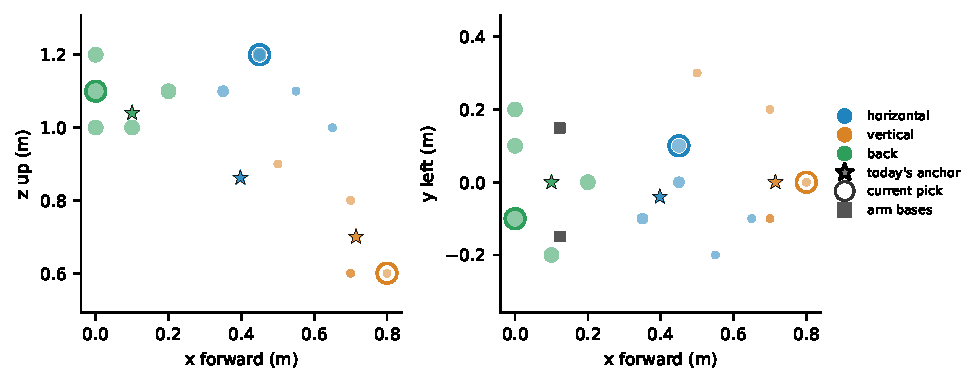
\includegraphics[width=\linewidth]{figures/prm_carry.pdf}
\caption{Stage-2 carry candidates by their grasp midpoint (side and top view; marker
size grows with the number of goals reached within 10\,mm). Stars: today's anchors;
rings: the current picks.}
\label{fig:carry}
\end{figure}

\paragraph{What the search says.} The carry \emph{class} matters more than the
exact place. Back carry is the best class: today's back anchor and the best back
candidate both reach 4 of the 14 goals with an exact path from a route within
10\,mm; moving it does not help much (the best candidate has a smaller median exact
gap, 5.6\,mm). Horizontal carry is where today's anchor is clearly wrong: it reaches
none of the 14 goals, while the best candidate, raised to $z = 1.2$\,m and moved
forward and left (midpoint $(0.45, 0.10, 1.20)$\,m, roll $60^\circ$), reaches 2
within 10\,mm and 4 with some exact path. No vertical pose works: the best reaches one
goal at 20\,mm. And for most goals no carry pose of any class reaches within 10\,mm on a
3000-node roadmap, which says the goals, not the carry poses, are the hard part at this
density. The current picks are in \path{asset/carry_poses.json}, marked
provisional, with the three best of each class listed for a person to choose from;
nothing in the planner or the library uses them yet.

\subsection{Precomputing overnight (E6)}
\label{sec:precompute}

The night before, only the bar and its grasps are known; the goal (the base's
parked pose relative to the structure) is known only on site. Everything that does
not depend on the goal can therefore move to the night: the roadmap itself, with
the three carry poses' branch pairs as nodes and every edge collision-checked, and
the exact tracking of every roadmap edge within 10\,mm (\code{prm_pilot.py track},
which writes the verdicts and waypoints to \path{tracked_10mm.json.gz}). Online, a
query only solves the goal pose and the three carry poses, measures their edges,
and searches; the refinement then tracks only the few edges that touch the goal
(\code{refine --pretracked}). The test uses goals the roadmap was \emph{not}
anchored on (B18 goals 2, 10, 20, 31, 47) and the provisional carry poses.

\begin{table}[h]
\centering
\footnotesize
\setlength{\tabcolsep}{3pt}
\caption{A night roadmap of 6000 nodes anchored on 17 other goals of B18 and the three
carry poses, then five online queries for unseen goals (8 workers). Worker start-up is
listed apart: a planner that runs for a whole session pays it once.}
\label{tab:precompute6k}
\begin{tabular}{@{}>{\raggedright\arraybackslash}p{6.4cm} rrrrr@{}}
\toprule
unseen goal & 2 & 10 & 20 & 31 & 47 \\
\midrule
night: nodes, of which anchors (count) & 6248, 248 &  &  &  &  \\
night: goals the roadmap is anchored on (count) & 17 &  &  &  &  \\
night: build time (s) & 821 &  &  &  &  \\
night: collision-free edges, of which within 10 mm (count) & 33582, 1218 &  &  &  &  \\
night: tracking the edges within 10 mm (s) & 151 &  &  &  &  \\
night: components of the free graph (count) & 318 &  &  &  &  \\
\midrule
online query: start the workers (s) & 9.8 & 10.0 & 9.6 & 10.0 & 10.0 \\
\quad solve the goal and the 3 carry poses (s) & 1.5 & 1.4 & 1.5 & 1.4 & 1.4 \\
\quad holding error of their edges (s) & 0.2 & 0.8 & 0.2 & 0.5 & 0.0 \\
\quad gaps, with lazy collision checks (s) & 0.1 & 0.2 & 0.1 & 0.3 & 0.1 \\
\quad whole query (s) & 16.5 & 16.4 & 15.4 & 15.9 & 15.2 \\
online refinement with the night's verdicts (s) & 12.0 & 12.1 & 11.6 & 11.7 & 12.1 \\
\quad of which starting its workers (s) & 9.9 & 10.1 & 9.7 & 9.8 & 10.0 \\
\midrule
best gap from the carry poses to the goal (mm) & 56.2 & 16.6 & 32.5 & 19.0 & $\infty$ \\
carry poses with an exact path within 10 mm (of 3) & 0 & 0 & 0 & 0 & 0 \\
\bottomrule
\end{tabular}

\end{table}

\paragraph{Online time is small; coverage is the problem.} Without the 10\,s of
worker start-up, an online query for an unseen goal took about 6\,s (most of it
reading the roadmap file; solving the 4 poses took 1.5\,s, the gaps 0.1--0.3\,s)
and the refinement about 2\,s (Table~\ref{tab:precompute6k}). But none of the five
unseen goals came within 10\,mm of a carry pose: best gaps of 17--56\,mm, and no
route at all to goal 47. A 6000-node roadmap spread over 17 goals is far sparser per
goal than the 4000 nodes the goal-2 roadmap spent on one goal, and only 1218 of its
33\,582 free edges are within 10\,mm. What the night has to buy is density, not
speed: Table~\ref{tab:precompute30k} repeats the test with a 30\,000-node roadmap
anchored on 45 goals.

\begin{table}[h]
\centering
\footnotesize
\setlength{\tabcolsep}{3pt}
\caption{The same test with a night roadmap of 30\,000 nodes anchored on the 45 other
goals of B18.}
\label{tab:precompute30k}
\IfFileExists{figures/prm_table_precompute_30k.tex}{\begin{tabular}{@{}>{\raggedright\arraybackslash}p{6.4cm} rrrrr@{}}
\toprule
unseen goal & 2 & 10 & 20 & 31 & 47 \\
\midrule
night: nodes, of which anchors (count) & 30494, 494 &  &  &  &  \\
night: goals the roadmap is anchored on (count) & 45 &  &  &  &  \\
night: build time (s) & 2128 &  &  &  &  \\
night: collision-free edges, of which within 10 mm (count) & 190571, 16883 &  &  &  &  \\
night: tracking the edges within 10 mm (s) & 5319 &  &  &  &  \\
night: components of the free graph (count) & 682 &  &  &  &  \\
\midrule
online query: start the workers (s) & 7.7 & 7.9 & 7.7 & 7.5 & 7.7 \\
\quad solve the goal and the 3 carry poses (s) & 1.3 & 1.1 & 1.4 & 1.2 & 1.2 \\
\quad holding error of their edges (s) & 0.3 & 0.5 & 0.3 & 0.3 & 0.0 \\
\quad gaps, with lazy collision checks (s) & 0.3 & 0.2 & 0.2 & 0.2 & 0.9 \\
\quad whole query (s) & 17.4 & 16.5 & 16.4 & 16.5 & 15.7 \\
online refinement with the night's verdicts (s) & 13.7 & 16.1 & 12.4 & 12.5 & 12.1 \\
\quad of which starting its workers (s) & 8.0 & 7.7 & 7.8 & 7.7 & 7.5 \\
\midrule
best gap from the carry poses to the goal (mm) & 40.2 & 9.8 & 11.7 & 13.1 & $\infty$ \\
carry poses with an exact path within 10 mm (of 3) & 0 & 1 & 0 & 0 & 0 \\
\bottomrule
\end{tabular}
}{(still running)}
\end{table}

\paragraph{A night-sized roadmap: closer, and the carry set becomes the limit.} The
30\,000-node roadmap took 35 minutes to build and 89 minutes to track its 16\,883 edges
within 10\,mm (16\,013 track), about two hours in all on eight workers; its largest
component holds 320 of the 405 goal anchors and 85 of the 88 carry-pose anchors. The
online cost stayed about the same (Table~\ref{tab:precompute30k}): about 16\,s per query,
of which 8\,s start the workers, 2\,s are the query's own phases and most of the rest is
reading the five-times larger roadmap file -- both would be paid once by a planner that
keeps its workers and the roadmap loaded for the session. Unseen goal 10 now has an
exact path (from a 9.8\,mm route; it passes the production repair), goals 20 and 31 come
within 12--13\,mm, goal 2 stays at 40\,mm and goal 47 has no route. Goal 2 is telling: the
all-starts query of Section~\ref{sec:e2} found routes of 2.9\,mm to it from the library's
back starts, but from the three fixed carry poses the best is 40\,mm. Fixing a single pose
per class gives up most of the start-set freedom that made the roadmap work; a small
family of carry poses per class (a few places and rolls), all in the night roadmap and
all in the online start set, costs nothing online and is the obvious next step.

\subsection{Bar B3}

\begin{table}[h]
\centering
\footnotesize
\caption{Bar B3, one 2000-node roadmap anchored on goals 4, 11 and 16; the three
night-1 starts of each goal. ``night 1'': seeds (of 10) the BiRRT solved.}
\label{tab:b3}
\begin{tabular}{@{}rrllrrrr@{}}
\toprule
goal & start & carry & class & night 1 & gap & lib. gap & best pair \\
\midrule
\tablerows{figures/prm_table_b3.tex}
\bottomrule
\end{tabular}
\end{table}

On bar B3 the roadmap orders the three night-1 starts of each goal as the BiRRT
did (Table~\ref{tab:b3}). In goal 4, start 42 (8 of 10 seeds) has a 6.5\,mm gap,
start 13 (4 of 10) 16.2\,mm, and start 0 (0 of 10) no route at all. In goal 16
the best-solved start (13, 8 of 10 seeds) has the smallest gap, 7.5\,mm, against
17.1\,mm for the other two. In goal 11, where starts 13 and 221 were each solved
twice, start 13 has 7.6\,mm and start 221 16.7\,mm. Start 0 --- production's
horizontal pick in all three goals --- has the largest gap or ties for it. Again the library configuration is rarely the best:
start 13 of goal 11 reaches the goals within 7.6\,mm on its best branch pair
but only within 35.6\,mm on its library configuration.

\subsection{What this says, and what it does not}

\paragraph{Observations.}
\begin{enumerate}[nosep,label=(\roman*)]
  \item \textbf{The pilot's two questions have first answers.} (1) On B18 goal 2,
        a joint-continuous path exists whose holding error stays under
        \PrmBestGap\,mm, from a start the BiRRT also solved, found with 4000
        nodes: 23\,024 IK calls (21\,408 to build, 1616 to solve the 808 endpoint
        poses) and 141\,501 collision checks (89\,047 to build, 52\,454 for the
        query over all 807 starts), in 232\,s plus 212\,s on eight workers. No
        path under 2\,mm was found at any budget. (2) Where the
        roadmap fails, the failure is local and of known shape: the best route's
        error is a row of similar peaks at 1--3\,mm, two edges over 2\,mm; start
        0's is a few long edges right next to the start.
  \item \textbf{The gap is a useful difficulty measure without running the BiRRT.}
        It separates the starts the BiRRT solved from those it did not
        (median 6.8 against 24.3\,mm), orders the library's classes, and on B3
        orders the night-1 starts of three goals as the BiRRT did.
  \item \textbf{The carry anchor, and the branch pair, are decided wrongly today.}
        For B18 goal 2 only back-carry starts come within 10\,mm, while
        production picks the horizontal anchor; and for 610 of 657 reachable
        starts some other branch pair or turn beats the library's own start
        configuration. A roadmap query over a set of starts makes both choices
        by search.
  \item \textbf{Global density is the wrong lever.} Doubling the node budget
        from 2000 to 4000 lowered the best gap from 4.2 to 2.9\,mm and did not
        reach any start that was unreachable at 1000. The holding error of an
        edge is set by its length (Fig.~\ref{fig:viol}), and random nodes do
        not shorten the edges of one particular route fast enough.
  \item \textbf{Collision checking is the cost.} 93\,\% of build worker time;
        IK is under 3\,\%. The work parallelises almost perfectly on the CPU
        (8.0x on 8 workers for edges). A GPU, if ever, would be for batched
        collision checks.
\end{enumerate}

\paragraph{What the numbers do not say.}
A gap is an upper bound on the smallest holding error a path needs: a denser or
better-placed roadmap can only lower it. ``Unreachable'' means unreachable in
this roadmap within $90^\circ$ edges, not infeasible ($90^\circ$ is the
largest move of any single joint along one edge, in either direction, so a
band of $180^\circ$; Section~\ref{sec:e1} widens it to $160^\circ$). Each budget was built once
(seed 0); at 2000 nodes a different seed moves the best gap by about 1\,mm and
the 30\,mm count by more than a factor of two (Table~\ref{tab:ablation}). Collision along an edge is checked every $10^\circ$ of joint motion,
coarser than the production planner's 2\,mm pose steps, so a roadmap path has
to be re-solved exactly (\code{core.repair_joint_path}, step 7 of the plan)
before it can be executed; the pilot does not do this yet. And all of this is
one goal of one bar, plus three goals of B3.

\paragraph{Second version: what the new experiments add.}
\begin{enumerate}[nosep,label=(\roman*),resume]
  \item \textbf{A 10\,mm roadmap route is nearly an exact path.} Tracking the bar
        along a route and solving both arms at every step turned 34 of the 36 routes
        within 10\,mm, and 245 of 462 within 30\,mm, into exact paths; all 245 pass
        the production repair unchanged. That is about twelve times the 21 starts the BiRRT
        solved, including 164 horizontal starts it never solved (Section~\ref{sec:e2}).
  \item \textbf{The hard part of exactness is branches, not millimetres.} Most
        edges that fail to track have a joint line through a stretched elbow, where
        the exact path ends on the mirror branch; and four rounds of the production
        check were needed to find every way a coarse chain can hop between branches
        near such a point (Section~\ref{sec:refine}).
  \item \textbf{Wider edges do not help; more branches help per draw}
        (Section~\ref{sec:e1}).
  \item \textbf{Carry poses: the class matters more than the place.} Back carry is
        best and today's back anchor is about as good as any; today's horizontal
        anchor reaches none of 14 goals, a raised one reaches 2--4; no vertical pose
        works (Section~\ref{sec:e5}).
  \item \textbf{Overnight precomputation makes the online part a few seconds}, but
        the night has to buy density: a 6000-node roadmap over 17 goals reached none
        of 5 unseen goals within 10\,mm (Section~\ref{sec:precompute}).
\end{enumerate}

\paragraph{Next steps suggested by the data.}
\begin{enumerate}[nosep]
  \item \textbf{Bring the refinement into the planner}: a \code{use_prm} variant of
        \code{plan_constrained_dual_arm} that queries a stored roadmap with the carry
        poses as the start set, refines, and hands the production repair a path, and
        a benchmark variant so it can be batched against the BiRRT.
  \item \textbf{Collision distance along the route}: the production check passes
        everything now, but only collisions at 1\,cm waypoints are checked during
        tracking; a clearance cost would keep routes away from contact.
  \item \textbf{Denser night roadmaps}: decide the node budget per goal region from
        the 30\,000-node test, and whether goals of one structure can share it.
  \item \textbf{Choose the carry poses} from the three listed per class, then
        re-run the night build with them.
\end{enumerate}
